\section{J. Pratt, Goswami - Capture Point: A Step toward Humanoid Push Recovery \cite{Pratt+CDG:2006}}
Authors: J. Pratt, Goswami\\
Year: 2006
\subsection*{Summary}
The Capture Point CP is defined for push recovery purposes, namely for determining how many steps must be performed by the biped robot to recover from a push. This is done on a simplified LIP +  Flywheel model as the whole body dynamics of a robot is too complicated (being it highly dimensional, nonlinear and \textbf{hybrid}). First of all the CP is computed using the LIP model only, so that the robot can only act on the linear force $f_k$ for the push recovery, this leads to a unique point CP. The addition of the Flywheel acts as a further degree of freedom of the simplified model, that can use both $f_k$ and $\tau$ to recover from the push. This leads to the computation of a \textbf{capture region}, namely the set of all the capture points.
\begin{figure}[h!]
  \centering
  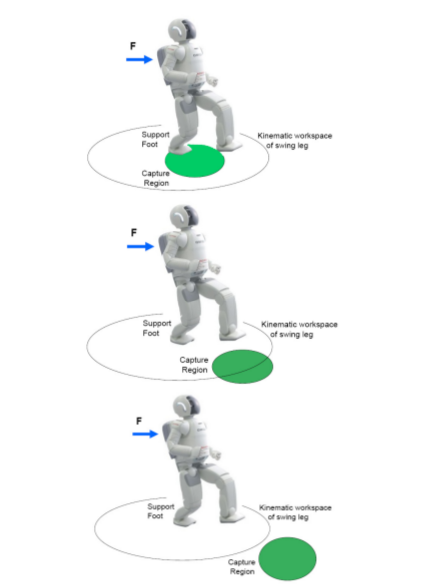
\includegraphics[width=90mm]{CapturePoint}
  \caption{The biped can recover from a push when its support polygon intersects the capture region}
\end{figure}
The different capture regions are computed for the following cases:
\begin{itemize}
\item Pure LIP model
\item LIP+Flywheel with instantaneous velocity variation
\item LIP+Flywheel with instantaneous position variation
\item LIP+Flywheel with limited torque and angle
\end{itemize}
\begin{figure}
  \centering
  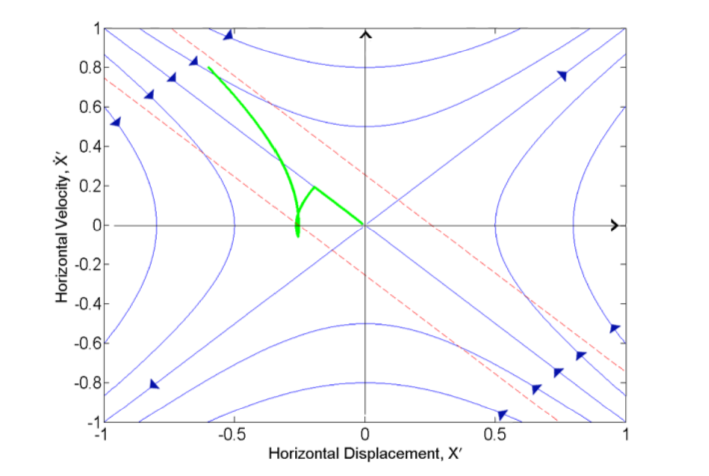
\includegraphics[width=90mm]{CPPhasePlane}
  \caption{Phase portrait of the LIP + Flywheel model}
  \label{PhasePlane}
\end{figure}
In figure \ref{PhasePlane} you can see here the trajectory of the x coordinate of the CoM starting from an arbitrary point and reaching a \textit{capture state} performing a \textit{safe feasible trajectory}. In the same figure also the capture region is represented with the red dotted line. You can see here that the green trajectory goes out of the capture region for a few instants, this is because the LIP+Flywheel as a non-null momentum in that points whereas the displayed capture region was computed for an initial state with null momentum.
\subsection*{Key points / Takeaways}
\begin{enumerate}
\item Closed-form expression of the CP for a LIP +  Flywheel model model 
\item Determining which is the best lunge profile to recover from the push, solving for example an optimization problem
\item The analysis of the capture region is carried out also with non-dimensional variables in order to detect the minimum number of variables needed.
\end{enumerate}
\subsection*{Weak points}
\begin{itemize}
\item What do the blue curves in the phase plane of figure \ref{PhasePlane} represent? \textbf{Answer}: they represent the evolution of the system in the autonomous case, when no external input is applied to the robot.
\end{itemize}
\subsection*{Ideas}
\begin{enumerate}
\item The definition of CP could be studied also for a SPRINGED LIP + Flywheel
\item How does the Phase Plane look like if we use the $(\dot{x},\ddot{x})$ variables? can we maybe in this case define a limit cycle and use the Poincar\'e return map for checking the system stability?
\end{enumerate}
